\chapter{Характеристика исходных данных курсового проекта}
\label{cha:ish_dannie}

\newcolumntype{Z}{>{\centering\arraybackslash}X}

\section{Исходные данные для проектирования}

Электрическая сеть сооружается в Костромской области на железобетонных опорах.

\begin{figure}[h]
	\centering
	\includegraphics[width=0.7\textwidth]{inc/svg/scheme}
	\caption{Схема расположения пунктов}
	\label{fig:scheme}
\end{figure}

Питание района электроэнергией будет осуществляться от шин 220 кВ подстанции "К" работающей в составе электроэнергетической системы. Источник питания в режиме наибольших нагрузок обеспечивает полную выдачу необходимой для потребителей активной мощности, а также 87 Мвар реактивной мощности. На шинах источника питания района в режиме наибольших нагрузок обеспечивается напряжение, равно 110 \%, а в режиме наименьших нагрузок 100 \% от номинального.

Для всех пунктов наименьшая нагрузка принимается 37 \% от наибольшей; число часов использования наибольших нагрузок составляет \(4350\; \frac{\textup{ч}}{\textup{год}}\).

Вторичное напряжение на всех сооружаемых подстанциях 10 кВ.

\section{Исходные данные по климатическим условиям и нагрузкам в пунктах потребления}

Среднеянварская температура: \(-11,8\; ^oC\)

Среднегодовая температура: \(2,7\; ^oC\)

Среднеиюльская температура: \(17,6\; ^oC\)

Ветровой район: I

Район по гололёду: I

Определим коэффициент реактивной мощности нагрузки \(\tg \, \varphi_\textup{нб1}\), потребляемую реактивную мощность \(Q_\textup{нб1}\) и полную мощность \(S_\textup{нб1}\) для пункта 1:
\[\tg \, \varphi_\textup{нб1} = \tg(\arccos(\cos\, \varphi_\textup{нб1})) = \tg(\arccos(0,92)) = 0,426\]
\[Q_\textup{нб1} = P_\textup{нб1} \cdot \tg\, \varphi_\textup{нб1} = 70 \cdot 0,426 = 29,8\; \textup{Мвар}\]
\[S_\textup{нб1} = \sqrt{P_\textup{нб1}^2 + Q_\textup{нб1}^2} = \sqrt{70^2 + 29,8^2} = 76,1\; \textup{МВА}\]

Сведем результаты расчета для всех пяти пунктов в таблицу \ref{tab:nagruzki}


\begin{table}[ht]
	\small
	\caption{Исходные данные по нагрузкам в пунктах потребления}
	\begin{tabularx}{\textwidth}{|X|Z|Z|Z|Z|Z|}
		\hline
		Пункт                             & 1     & 2     & 3     & 4     & 5     \\ \hline
		$P_\textup{нб},\; \textup{МВт}$   & 70    & 70    & 30    & 40    & 35    \\ \hline
		$\cos\, \varphi_\textup{нб}$      & 0,92  & 0,92  & 0,91  & 0,89  & 0,91  \\ \hline
		$\tg\, \varphi_\textup{нб}$       & 0,426 & 0,426 & 0,456 & 0,512 & 0,456 \\ \hline
		$Q_\textup{нб}, \; \textup{Мвар}$ & 29,8  & 29,8  & 13,7  & 20,5  & 16,0  \\ \hline
		$S_\textup{нб}, \; \textup{МВА}$  & 76,1  & 76,1  & 33,0  & 44,9  & 38,5  \\ \hline
	\end{tabularx}
	\label{tab:nagruzki}
\end{table}

\section{Определение длин пролётов}
Определим длины воздушных линий между пунктами и сведем результаты в таблицу \ref{tab:dlina}
\begin{table}[H]
	\small
	\caption{Расстояние между пунктами $l_{ij(m)}$, в клеточках}
	\begin{tabularx}{\textwidth}{|X|Z|Z|Z|Z|Z|Z|}
		\hline
		Пункты & К    & 1     & 2     & 3     & 4     & 5     \\ \hline
		К      & "--- & 3,606 & 4,243 & "---  & "---  & "---  \\ \hline
		1      &      & "---  & 5     & 4,243 & 5,385 & "---  \\ \hline
		2      &      &       & "---  & 3,606 & "---  & "---  \\ \hline
		3      &      &       &       & "---  & 2,236 & 4     \\ \hline
		4      &      &       &       &       & "---  & 2,236 \\ \hline
		5      &      &       &       &       &       & "---  \\ \hline
	\end{tabularx}
	\label{tab:dlina}
\end{table}

Протяженность намечаемых воздушных линий при отсутствии точных данных рекомендуется принимать с учетом удлинения трасс линий (по сравнению с наикратчайшим расстоянием между пунктами по воздушной прямой) за счет их непрямолинейности:
\begin{eqndesc}[H]
	\begin{equation}
		L_{ij} = l_{ij} k_\textup{удл},
	\end{equation}

	где $L_{ij}$ "--- длина воздушной линии между пунктами i и j, км; \\
	$l_{ij}$ "--- наикратчайшее расстояние между пунктами i и j по воздушной прямой, км; \\
	$k_\textup{удл}$ "--- коэффициент удлинения трассы воздушной линии (табл. \ref{tab:k_udl}).
\end{eqndesc}

\begin{table}[H]
	\small
	\caption{Коэффициенты удлинения трассы воздушных линий ($k_\textup{удл}$)}
	\begin{tabularx}{\textwidth}{|X|Z|Z|Z|Z|Z|Z|Z|}
		\hline
		Регион           & Центр & Северо-Запад & Северный Кавказ & Средняя Волга & Урал & Сибирь & Восток \\ \hline
		$k_\textup{удл}$ & 1,16  & 1,20         & 1,26            & 1,16          & 1,16 & 1,20   & 1,20   \\ \hline
	\end{tabularx}
	\label{tab:k_udl}
\end{table}
Для Костромы (Центр) $k_\textup{удл} = 1,16$ 

Наикратчайшее расстояние между пунктами i и j по воздушной прямой пересчитаем в масштабе по формуле:
\[l_{ij} = l_{ij(m)} \cdot m\]

Соотношение масштаба m равно 1:10. Тогда пересчитаем длины воздушных линий между пунктами и сведем результаты в таблицу \ref{tab:dlina_pereschet}
\begin{table}[H]
	\small
	\caption{Расстояние между пунктами $L_{ij}$, км}
	\begin{tabularx}{\textwidth}{|X|Z|Z|Z|Z|Z|Z|}
		\hline
		Пункты & К    & 1    & 2    & 3    & 4    & 5    \\ \hline
		К      & "--- & 41,8 & 49,2 & "--- & "--- & "--- \\ \hline
		1      &      & "--- & 58,0 & 41,8 & 62,5 & "--- \\ \hline
		2      &      &      & "--- & 41,8 & "--- & "--- \\ \hline
		3      &      &      &      & "--- & 25,9 & 46,4 \\ \hline
		4      &      &      &      &      & "--- & 25,9 \\ \hline
		5      &      &      &      &      &      & "--- \\ \hline
	\end{tabularx}
	\label{tab:dlina_pereschet}
\end{table}

\section{Оценка суммарной активной мощности, потребляемой в проектируемой сети, и значения коэффициентов реактивной мощности}
При определении одновременно потребляемой активной мощности (с учетом наибольших нагрузок пунктов потребления и потерь активной мощности в элементах электрической сети) следует учитывать несовпадения по времени суток наибольших нагрузок (НБ) отдельных потребителей. При перспективном проектировании, когда точные графики нагрузок потребителей неизвестны, используют среднестатистические значения  коэффициентов одновременности нагрузок. Таким образом, суммарая активная мощность, потребляемая в проектируемой сети, составляет:
\begin{eqndesc}[H]
	\begin{equation}
		P_{\textup{треб}\Sigma} = k_\textup{однP} \cdot \sum^n_{i=1} P_{\textup{нб}i} + \Dap_* \cdot \sum^n_{i=1} P_{\textup{нб}i},
	\end{equation}
	где $P_{\textup{нб}i}$ "--- наибольшая активная нагрузка \textit{i}-го пункта потребления; \\
	\textit{n} "--- число пунктов потребления электроэнергии; \\
	$k_\textup{однP}$ "--- коэффициент одновременности наибольших активных нагрузок подстанций; \\
	${\displaystyle \Dap_*}$ "--- суммарные потери активной мощности в элементах сети в долях от суммарной нагрузки подстанций.
	\label{eqn:p_treb_sum}
\end{eqndesc}
%%% Local Variables:
%%% mode: latex
%%% TeX-master: "rpz"
%%% End: